\chapter{Υλοποίηση Συστήματος}
\label{chap5}

Μέχρι στιγμής, έχει γίνει αναφορά στις τεχνολογίες και τις τεχνικές σχεδίασης της εφαρμογής. Το κεφάλαιο αυτό επεκτείνεται στην υλοποίηση της εφαρμογής, αναλύοντας τις μεθόδους που χρησιμοποίηθηκαν για τον προγραμματισμό τόσο του \tl{frontend}, όσο και του \tl{backend}. Η ενότητα 5.1 αφορά το \tl{frontend} κομμάτι, δηλαδή με τον προγραμματισμό των διεπιφανειών χρήστη. Η ενότητα 5.2 καταπιάνεται με την υλοποίηση του \tl{backend}, το οποίο απαρτίζεται από τον εξυπηρετητή αιτημάτων που δημιουργούνται από τις διεπιφάνειες χρήστη και τη βάση δεδομένων στην οποία αποθηκεύονται όλες οι πληροφορίες της εφαρμογής. Στην ενότητα 5.3 παρουσιάζονται τα τεχνολογικά εργαλεία τα οποία χρειάστηκαν στην υλοποίηση. Τέλος, στην ενότητα 5.4 γίνεται μια συνοπτική αναφορά στην πλοτφόρμα προγραμματισμού που επιλέχθηκε για την υλοποίηση της εφαρμογής. 


\section{Λεπτομέρειες Υλοποίησης Διεπιφανειών Χρήστη}
Ιδιαίτερο ενδιαφέρον παρουσιάζουν οι τεχνικές που χρησιμοποιήθηκαν στην υλοποίηση του συστήματος διεπιφανειών χρήστη. Η εφαρμογή αφορά κινητές συσκευές με λειτουργικό \tl{iOS}, επομένως δόθηκε μεγάλη βαρύτητα σε μεθόδους που υιοθετούν οι περισσότερες \tl{native} εφαρμογές της ίδιας κατηγορίας. Κατά τον προγραμματισμό, σχεδόν όλες οι διεπαφές που χρησιμοποιούνται αφορούν αποκλειστικά \tl{iOS} πλατφόρμες προκειμένου να προσφέρουν την καλύτερη δυνατή εμπειρία στο χρήστη.
\newline
\indent
Η εφαρμογή αναφέρεται σε κινητά τελευταίας γενιάς. Αυτό εισάγει κάποιους περιορισμούς στον προγραμματισμό, αλλά έχει ταυτοχρόνως και κάποια πλεονεκτήματα. Για παράδειγμα, οι διαστάσεις της οθόνης στις κινητές συσκευές είναι πολύ μικρότερες από αυτές ενός σταθερού υπολογιστή. Διαδραστικά στοιχεία όπως πλήκτρα, πεδία εισόδου, εικονίδια και άλλα γραφικά θα πρέπει να λαμβάνουν υπόψη τους τον παραπάνω περιορισμό. Συνεπώς, ο προγραμματισμός για \tl{mobile apps} είναι σαφώς πιο δύσκολος από τον προγραμματισμό για \tl{desktop apps}. 
\newline
\indent
Το κυριότερο πλεονέκτημα του προγραμματισμού για να \tl{mobile apps} είναι το γεγονός ότι δεν χρειάζεται να δωθεί ιδιαίτερη βάση σε λεπτομέρειες, αφού οι οθόνες των κινητών δεν επιτρέπουν την σχολαστική ενασχόληση με κάθε στοιχείο ή την υπερβολική λεπτομέρεια των διαδραστικών στοιχείων, αφού αυτό θα καθιστούσε την εμπειρία χρήσης της εφαρμογής κουραστική για το χρήστη. Έτσι, ο προγραμματισμός επικεντρώνεται κυρίως γύρω από το κομμάτι με το οποίο θα αλληλιπιδρά ο χρήστης και τις τεχνικές λεπτομέρειες που συμπεριλαμβάνει. Για να εξασφαλιστεί μια ολοκληρωμένη, αλλά συγχρόνως απλή εμπειρία εντός της εφαρμογής, όλες οι διεπιφάνειες ακολουθούν αυτή την τακτική, όπου το διαδραστικό περιβάλλον αποτελείται αποκλειστικά από διεπαφές που είναι ζωτικές για την σωστή λειτουργία της κάθε οθόνης.


\subsection{Βασικά Προγραμματιστικά Χαρακτηριστικά Οθονών}
Μιλάω για τα τμήματα ζωτικής σημασίας που έχουν οι περισσότερες οθόνες..

\subsubsection{Τεχνική Πλοήγησης στην Εφαρμογή}



\subsubsection{Επικεφαλίδα Οθόνης}



\subsubsection{Κεντρικό Μενού Οθονών}



\subsubsection{Βασικά Πλήκτρα Ενεργειών}



\subsection{Λειτουργικότητα Οθονών Εφαρμογής}



\subsubsection{\tl{WelcomeScreen}}


\subsubsection{\tl{RegisterScreen}}


\subsubsection{\tl{LoginScreen}}


\subsubsection{\tl{HomeScreen}}


\subsubsection{\tl{CreateHotspotScreen}}



\subsubsection{\tl{HotspotListScreen}}


\subsubsection{\tl{CommentScreen}}


\subsubsection{\tl{ProfileScreen}}


\subsection{Τενικές Ενιαίας Διαχείρισης Δεδομένων}



\subsubsection{\tl{React Redux}}



\subsubsection{\tl{Redux Thunk Middleware}}




\subsection{Βιβλιοθήκες και Βοηθητικά Προγραμματιστικά Πακέτα}





\subsection{Ιεράρχηση Αρχείων και Δομή Φακέλων}

\section{Σύστημα αξιολόγησης}

Εδώ περιγράφουμε το σύστημα που χρησιμοποιήσαμε για να αξιολογήσουμε τις τεχνικές μας. Συνήθως, η περιγραφή γίνεται με κείμενο και με ένα block diagram περιγραφής των λειτουργιών του συστήματος.
Αν το σύστημα είναι μεγάλο, τότε συζητήστε με τον επιβλέποντα μήπως χρειάζεται να υπάρχει ξεχωριστό κεφάλαιο με τίτλο ` Σχεδίαση συστήματος '. 

\section{Οργάνωση πειραμάτων}

Εδώ περιγράφουμε λεπτομερώς πώς οργανώσαμε τα πειράματα. Π.χ.
α) τί σύνολο δεδομένων χρησιμοποιήσαμε (συνθετικά, έτοιμες συλλογές)
β) τί τιμές είχαν διάφοροι παράμετροι του συστήματός αξιολόγησης, κ.λ.π.

Οι τιμές των παραμέτρων μπορούν να φαίνονται και σε πίνακα, όπως λ.χ. στον Πίνακα \ref{tab:parameters}:

\begin{table}[h]
\centering
\begin{tabular}{|c|>{\centering\arraybackslash}m{8cm}|}
\hline Πλήθος κελιών καννάβου \textit{\tl{c}} $\times$ \textit{\tl{c}} & 50 $\times$ 50, 100 $\times$ 100, 200 $\times$ 200, \textbf{250} $\times$ \textbf{250}, 500 $\times$ 500, 1000 $\times$ 1000  \\
\hline Τυπική απόκλιση $\sigma$ & 25\tl{m}, 50\tl{m}, 75\tl{m}, \textbf{100\tl{m}}, 150\tl{m}, 200\tl{m} \\
\hline Αριθμός εγγύτερων γειτόνων \textit{\tl{k}} & 1, 2, \textbf{3}, 4, 5, 10, 20 \\
\hline Πιθανοτικό κατώφλι $\theta$ & 50$\%$, 60$\%$, 70$\%$, \textbf{75$\%$}, 80$\%$, 90$\%$, 99$\%$ \\
\hline  
\end{tabular}
\caption{Παράμετροι πειραμάτων}
\label{tab:parameters}
\end{table}

Αν χρησιμοποιήσατε συνθετικά δεδομένα, τότε εξηγήστε στην παρακάτω χωριστή υποενότητα τον τρόπο που τα δημιουργήσατε:

\subsection{Παραγωγή συνθετικών δεδομένων}

Τα πειραματικά δεδομένα παρήχθησαν ...


\section{Αποτελέσματα της μελέτης}

Εδώ παρουσιάζουμε τα αποτελέσματα των μετρήσεων με μορφή γραφικών παραστάσεων, όπως ενδεικτικά στο Σχ. \ref{GridGranularity}. Δίνουμε λεπτομερή εξήγηση και σχολιασμό των αποτελεσμάτων, πάντα σε σχέση με το πρόβλημα που οι τεχνικές μας φιλοδοξούν να λύσουν. 
Φροντίστε να ομαδοποιήσετε τα αποτελέσματα (σε χωριστές υποενότητες)ανάλογα με τις παραμέτρους που μετράτε, π.χ. χωριστά το κόστος σε χρόνο από το κόστος σε χώρο ή όσον αφορά την ακρίβεια των απαντήσεων.

\begin{figure}[t!]
\includegraphics[scale=0.5]{figures/grid_granularity.eps}
\centering
\caption{Κλιμάκωση χρόνου εκτέλεσης για διάφορες υποδιαιρέσεις του καννάβου}	
\label{GridGranularity}
\end{figure} 


\section{Σύνοψη συμπερασμάτων αξιολόγησης}

Εδώ συνοψίζουμε τα συμπεράσματα της αξιολόγησης. Η σύνοψη να γίνεται σύντομα και καθαρά, π.χ. 1. αυτό, 2. το άλλο, κ.ο.κ.


%Αυτά που ακολοθούν θα μπουν στο Κεφ. 5 

\subsubsection{\tl{Server Routes}}

Ο \tl{server} χρησιμοποιεί ένα σύστημα δρομολόγησης (\tl{routes}) των αιτημάτων του \tl{client} που προορίζονται προς εξυπηρέτηση. Κάθε ομάδα υπηρεσιών που απευθύνονται σε μια συγκεκριμένη λειτουργία της εφαρμογής αντιστοιχίζεται σε ένα δρομολογητή (\tl{router}). Ο \tl{router} απαρτίζεται από επιμέρους \tl{routes}, καθεμία εκ των οποίων εξυπηρετεί μια συγκεκριμένη λειτουργία. Έτσι, στο παραπάνω παράδειγμα, το αίτημα για τη δημιουργία νέου \tl{hotspot} θα δρομολογηθεί για εξυπηρέτηση από τον \tl{router} που είναι υπεύθυνος για τις ενέργειες΄που αφορούν ένα \tl{hotspot} (\tl{\textit{HotspotRoutes}}). 

Το σύστημα των δρομολογητών έχει σχεδιαστεί με στόχο την απλότητα και την αμεσότητα στην κατανόηση από τον προγραμματιστή (βλ. Σχ. \ref{routes}). Αιτήματα που αφορούν τους χρήστες δρομολογούνται προς εξυπηρέτηση από τον \tl{router} που είναι υπεύθυνος για τις ενέργειες που αφορούν τους χρήστες. Με τον ίδιο τρόπο, Αιτήματα που σχετίζονται με σχόλια χρηστών σε ένα \tl{hotspot}, εξυπηρετούνται από εκείνο τον \tl{router} που είναι υπεύθυνος για τα σχόλια. 

\begin{figure}[h]
    \centering
    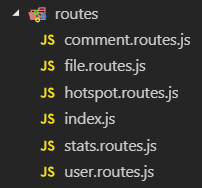
\includegraphics[scale=1]{figures/routes.png}
    \caption{Ιεράρχηση του συστήματος δρομολογητών στην εφαρμογή.}
    \label{routes}
\end{figure}

Οι δρομολογητές του συστήματος είναι οι ακόλουθοι:

\begin{itemize}
    \item \tl{\textbf{Hotspot Routes --}} περιλαμβάνει \tl{routes} που αφορούν την εξυπηρέτηση αιτημάτων σχετικά με \tl{hotspots}, όπως δημιουργία, επεξεργασία, διαγραφή, προβολή, ανάκτηση κλπ.
    \item \tl{\textbf{User Routes --}} περιλαμβάνει \tl{routes} που αφορούν την εξυπηρέτηση αιτημάτων σχετικά με χρήστες, όπως εγγραφή, σύνδεση, επεξεργασία, προβολή, ανάκτηση κλπ.
    \item \tl{\textbf{Comment Routes --}} περιλαμβάνει \tl{routes} που αφορούν την εξυπηρέτηση αιτημάτων σχετικά με σχόλια, όπως δημιουργία, προβολή, απαρίθμηση κλπ.
    \item \tl{\textbf{File Routes --}} περιλαμβάνει \tl{routes} που αφορούν την εξυπηρέτηση αιτημάτων σχετικά με συνημμένα αρχεία σε \tl{hotspots}.
    \item \tl{\textbf{Stats Routes --}} περιλαμβάνει \tl{routes} που αφορούν την εξυπηρέτηση αιτημάτων σχετικά με στατιστικά δεδομένα.
\end{itemize}

\subsubsection{\tl{Server Controllers}}

Αφότου τα αιτήματα δρομολογηθούν προς εξυπηρέτηση στους αντίστοιχους \tl{routers}, ακολοθεί η επεξεργασία τους και η εκτέλεσή τους μέσω κατάλληλων μεθόδων. Οι μέθοδοι που αναλαμβάνουν την εκτέλεση των αιτημάτων ονομάζονται ελεγκτές (\tl{controllers}) και αποτελούνται από ένα σύνολο ασύγχρονων εντολών και κλήσεων μεταξύ της βάσης δεδομένων και του \tl{server}.

Όπως και με το σύστημα των δρομολογητών, έτσι και οι ελεγκτές έχουν σχεδιαστεί με στόχο να αποσυμπλέκουν τις ενέργειες που σχετίζονται με κάθε αίτημα (βλ. Σχ. \ref{}). Όλες οι ενέργεεις που αφορούν τα \tl{hotspots} εκτελούνται αποκλειστικά από έναν ελεγκτή. Το ίδιο συμβαίνει και με τις ενέργεεις γύρω από τους χρήστες. Το σύστημα των \tl{controllers} έχει παραπλήσια μορφή με αυτό των \tl{routers} καθώς στόχος της σχεδίασης είναι να υπάρχει ένας βαθμός αναλογίας μεταξύ των διαφόρων τμημάτων,ο οποίος μειώνει αισθητά το χρόνο κατανόησης και βελτιστοποιεί τη διαδικασία υλοποίησης:

\begin{itemize}
    \item \tl{\textbf{Hotspot Controller --}} περιλαμβάνει τις μεθόδους που αφορούν την εξυπηρέτηση αιτημάτων σχετικά με \tl{hotspots}, όπως δημιουργία, επεξεργασία, διαγραφή, προβολή, ανάκτηση κλπ.
    \item \tl{\textbf{User Controller --}} περιλαμβάνει τις μεθόδους που αφορούν την εξυπηρέτηση αιτημάτων σχετικά με χρήστες, όπως εγγραφή, σύνδεση, επεξεργασία, προβολή, ανάκτηση κλπ.
    \item \tl{\textbf{Comment Controller --}} περιλαμβάνει τις μεθόδους που αφορούν την εξυπηρέτηση αιτημάτων σχετικά με σχόλια, όπως δημιουργία, προβολή, απαρίθμηση κλπ.
    \item \tl{\textbf{File Controller --}} περιλαμβάνει τις μεθόδους που αφορούν την εξυπηρέτηση αιτημάτων σχετικά με συνημμένα αρχεία σε \tl{hotspots}.
    \item \tl{\textbf{Stats Controller --}} περιλαμβάνει τις μεθόδους που αφορούν την εξυπηρέτηση αιτημάτων σχετικά με στατιστικά δεδομένα.
    \item \tl{\textbf{Views Controller --}} περιλαμβάνει τις μεθόδους που αφορούν την εξυπηρέτηση αιτημάτων σχετικά με τα \tl{views} ενός \tl{hotspot}.
\end{itemize}

